\documentclass[journal]{IEEEtran}
\usepackage[a5paper, margin=10mm, onecolumn]{geometry}
\usepackage[cmex10]{amsmath}
\usepackage{amssymb,amsfonts,amsthm}
\usepackage{gvv-book}
\usepackage{gvv}
\usepackage{hyperref}
\usepackage{physics}

\begin{document}


\title{2.10.54}
\author{EE25BTECH11025 - Ganachari Vishwambhar}
\maketitle

\textbf{Question}:\newline
Let $\vec{a, b,c}$ be unit vectors such that $\vec{a}+\vec{b}+\vec{c}=\vec{0}$. Which of the following are correct?\\
\begin{enumerate}
    \item $\vec{a}\times \vec{b}=\vec{b}\times \vec{c}=\vec{c}\times \vec{a}=\vec{0}$
    \item $\vec{a}\times \vec{b}=\vec{b}\times \vec{c}=\vec{c}\times \vec{a}\neq \vec{0}$
    \item $\vec{a}\times \vec{b}=\vec{b}\times \vec{c}=\vec{a}\times \vec{c}\neq \vec{0}$
    \item $\vec{a}\times \vec{b},\vec{b}\times \vec{c}, \vec{c}\times \vec{a}$ are mutually perpendicular.
\end{enumerate}
\textbf{Solution: }\\

Given:
\begin{align}
    \vec{a}+\vec{b}+\vec{c}=0\\
    \vec{c}= \myvec{\vec{a}&\vec{b}}\myvec{-1\\-1}\\
\end{align}

This $\vec{c}$ lies in span of $\vec{a}, \vec{b}$.\\

Since $\vec{a}, \vec{b}, \vec{c}$ are all in 2D space, if all three are non-zero unit vectors satisfying this relation, they must be linearly dependent.\\

Therefore, the $2\times2$ matrix $\myvec{\vec{a}&\vec{b}}$ cannot be invertible.
\begin{align}
    \mdet{\myvec{\vec{a}&\vec{b}}}=0
\end{align}

So the matrix is singular.

In 2D, norm is defined by the determinant:
\begin{align}
    ||\vec{a}\times\vec{b}||=\mdet{\myvec{\vec{a}&\vec{b}}}
\end{align}

So if $\mdet{\myvec{\vec{a}&\vec{b}}}=0$, then
\begin{align}
    \vec{a}\times\vec{b}=0
\end{align}

Similarly, we can show the same for the vectors $\vec{a}$ and $\vec{b}$.

Thus, the correct option is (1):
\begin{align}
    \vec{a}\times \vec{b}=\vec{b}\times \vec{c}=\vec{c}\times \vec{a}=\vec{0}
\end{align}



\begin{figure}[h!]
   \centering
   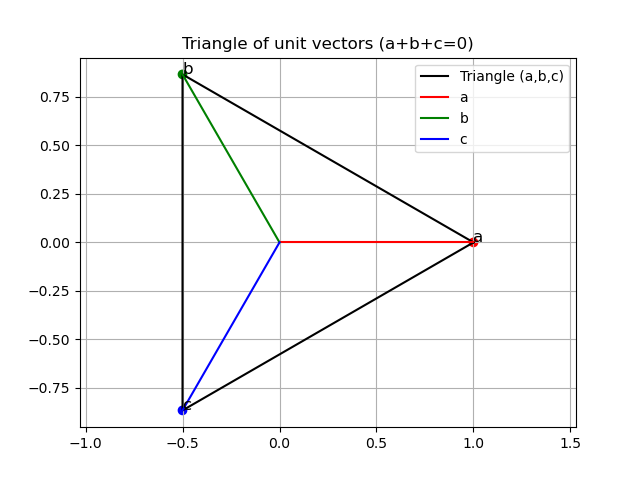
\includegraphics[width=0.7\linewidth]{figs/plot.png}
   \caption{Plot of the vectors $\vec{a}, \vec{b}$ and $\vec{c}$}
   \label{}
\end{figure}
\end{document}  
